\documentclass[12pt,letterpaper]{article}


\newcommand{\studentname}{Ben Bassett}
\newcommand{\labpartner}{Katrina Sumarli}

\title{\textsc{Lab 03: Standing Waves on a Cord}}
\newcommand{\shorttitle}{Harmonic Oscillator with Drag}

\newcommand{\course}{PHY310}
\newcommand{\labdate}{09-24-2024}

%------------------------------------------------------------------------------------------------------------

\usepackage[letterpaper,left=1in,right=1in,bottom=1in,top=1in]{geometry}
\usepackage{fancyhdr}
\usepackage{subfigure}
\usepackage{graphicx}
\usepackage{amsmath}
\usepackage{cleveref}
\usepackage{booktabs}
\usepackage[british]{babel}
\usepackage[square,comma,numbers,sort&compress]{natbib}
\usepackage{csvsimple}
\usepackage{graphicx}
\usepackage{pgfplotstable}
\usepackage{textcomp,gensymb}
\usepackage{array}
\usepackage{tabu}
\usepackage{multirow}
\usepackage{url}
\usepackage{lipsum}
\usepackage{dsfont}
\pgfplotsset{compat=1.9}% supress warning
\begin{document}

%------------------------------------------------------------------------------------------------------------

\setlength{\parindent}{1em}
\setlength{\parskip}{0.5em}
\author{\course~Lab Journal \\ \\ \studentname\,\& \labpartner}
\date{\labdate}

\renewcommand\abstractname{Summary}

\pagestyle{fancy}
\fancyhead{}
\fancyhead[l]{\course:~\shorttitle}
\fancyhead[r]{\studentname}
\fancyfoot{}
\fancyfoot[C]{\thepage}
\renewcommand{\headrulewidth}{0pt}
\renewcommand{\footrulewidth}{0pt}

\renewcommand\bibname{References}

%------------------------------------------------------------------------------------------------------------

\renewcommand\abstractname{Abstract}
\maketitle

% COMMENT IN IF ASKED TO SUBMIT REPORT WITH ABSTRACT
%\begin{abstract}
%Maximum 200 words.
%\end{abstract}

\section{Purpose}
This lab aimed to determine the velocity of waves on a string under tension, and the factors that affect this speed.

\section{Experimental Apparatus}

We were given a length of string, a mechanical wave driver, a mounted retort stand, a pulley, a black background, ruler, and various weights (including hanger). Our general setup is illustrated in Figure \ref{fig:setup}.

\begin{figure}[h]
    \centering
    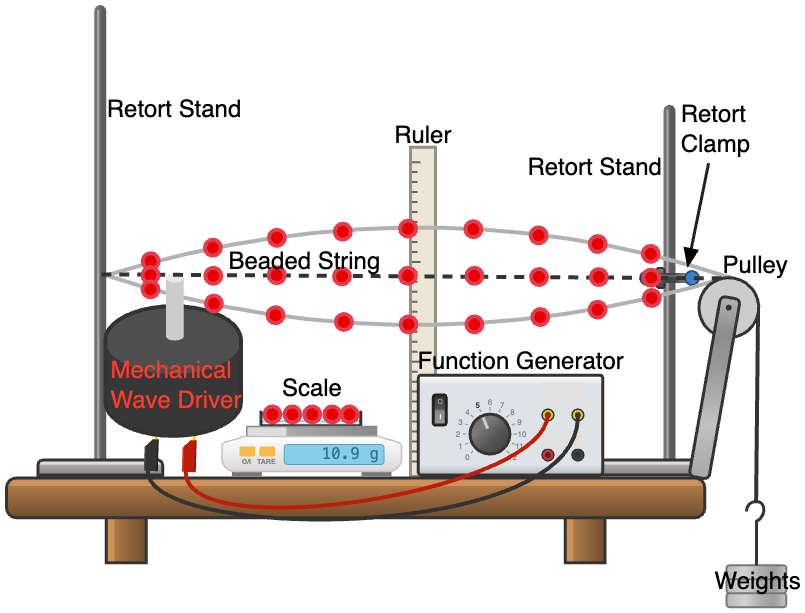
\includegraphics[width=4in]{images/setup.png}
    \caption{A diagram of our experimental setup}
    \label{fig:setup}
\end{figure}

% \pagebreak
\section{Procedure}

To begin, we tested our function generator to ensure that it was properly calibrated. To do so, we attached our voltage probe to the output of the function generator and to the LabQuest. We then measured a ~5 seconds of data at 1 Hz, 10 Hz, and 100 Hz at 6 V.

After this calibration, we tied one end of our string to the retort stand, and attempting to keep it level, we looped the other end over the pulley and tied on the weight hanger with 35 grams of weight (0.343 N of tension). We then placed the mechanical wave driver under the string so that the string rested in a notch in the driver's pronged extension. We then turned the function generator to 10 V and on the sine setting incremented by individual Hertz until the waves on the string appeared relatively stationary. We then incremented by tenths and hundredths of a Hertz until the amplitude of the wave seemed largest, and recorded the amplitude in mm with a ruler. We did this for standing waves $n=1$ through $n=6$.

After finding $n=\{1\dots 6\}$ with 0.343 N of tension, we found the $n=2$ state (easiest to visualize and measure amplitude for) at 35 g, 100 g, 150 g, 200 g, 250 g, 300 g, and 335 g of weight.

\section{Results}

We measured standing waves $n=\{1\dots 6\}$ with 35 g of weight. See that data in Table \ref{tab:35g}. The wavelength was not directly measured, but we measured the length of the entire string to be 153 cm and simply divided by $n$. To find the velocity of the wave, we can use the fact that $v=\lambda f$, and use the error propagation formula to calculate our errors:

\begin{equation}
    \delta f^2=\sum_i \left(\frac{\delta f}{\delta a_i}\right)^2\delta a_i^2
\end{equation}

\begin{equation*}
    \delta v = \sqrt{\left(\frac{\delta v}{\delta f}\right)^2 \times 0.001 \text{ m}^2 + \left(\frac{\delta v}{\delta \lambda}\right)^2 \times 0.01 \text{ m}^2}=\sqrt{\left(\lambda\right)^2 \times 0.001 \text{ m}^2 + \left(f\right)^2 \times 0.01 \text{ m}^2}
\end{equation*}

\begin{table}[ht]
\centering
\begin{tabular}{lllll}
                           & Frequency                            & Amplitude                       & Wavelength                       & Velocity                              \\ \cline{2-5} 
\multicolumn{1}{l|}{$n=1$} & \multicolumn{1}{l|}{13.67 ± 0.01 Hz} & \multicolumn{1}{l|}{21 ± 1 mm}  & \multicolumn{1}{l|}{153 ± 1 cm}  & \multicolumn{1}{l|}{209.2 ± 0.2 m/s} \\ \cline{2-5} 
\multicolumn{1}{l|}{$n=2$} & \multicolumn{1}{l|}{26.48 ± 0.01 Hz} & \multicolumn{1}{l|}{9.5 ± 1 mm} & \multicolumn{1}{l|}{76.5 ± 1 cm} & \multicolumn{1}{l|}{202.7 ± 0.2 m/s} \\ \cline{2-5} 
\multicolumn{1}{l|}{$n=3$} & \multicolumn{1}{l|}{40.54 ± 0.01 Hz} & \multicolumn{1}{l|}{8.0 ± 1 mm} & \multicolumn{1}{l|}{51.0 ± 1 cm} & \multicolumn{1}{l|}{206.8 ± 0.2 m/s} \\ \cline{2-5} 
\multicolumn{1}{l|}{$n=4$} & \multicolumn{1}{l|}{54.58 ± 0.01 Hz} & \multicolumn{1}{l|}{5.5 ± 1 mm} & \multicolumn{1}{l|}{38.3 ± 1 cm} & \multicolumn{1}{l|}{209.0 ± 0.2 m/s} \\ \cline{2-5} 
\multicolumn{1}{l|}{$n=5$} & \multicolumn{1}{l|}{68.37 ± 0.01 Hz} & \multicolumn{1}{l|}{3.5 ± 1 mm} & \multicolumn{1}{l|}{30.6 ± 1 cm} & \multicolumn{1}{l|}{209.2 ± 0.2 m/s} \\ \cline{2-5} 
\multicolumn{1}{l|}{$n=6$} & \multicolumn{1}{l|}{82.07 ± 0.01 Hz} & \multicolumn{1}{l|}{2.5 ± 1 mm} & \multicolumn{1}{l|}{25.5 ± 1 cm} & \multicolumn{1}{l|}{209.3 ± 0.2 m/s} \\ \cline{2-5} 
\end{tabular}
\label{tab:35g}
\caption{Resonances of string with 0.343 N of tension}
\end{table}

The frequency data very obviously follows a linear relationship, and is easily approximated as $f_n=n13.67$ Hz. See the data graphed in Figure \ref{fig:frequency}, fitted to a line with a slope that is the same value as the frequency at $n=1$, and has an $R^2$ of 1.00! 

\begin{figure}[h]
    \centering
    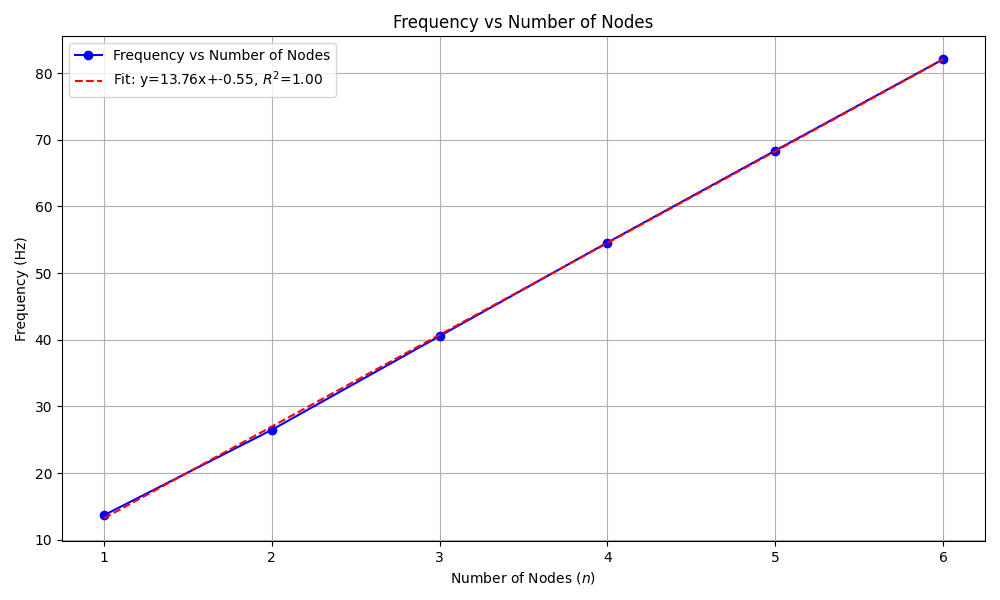
\includegraphics[width=4in]{images/frequency1-6.png}
    \caption{Frequency at $n=\{1\dots6\}$}
    \label{fig:frequency}
\end{figure}

However, I'm not sure what the relationship, if any, is from frequency to amplitude. It could be a decreasing exponential, but I have no theory to back up that claim, so no fit line is shown in Figure \ref{fig:amplitude}.

\begin{figure}[h]
    \centering
    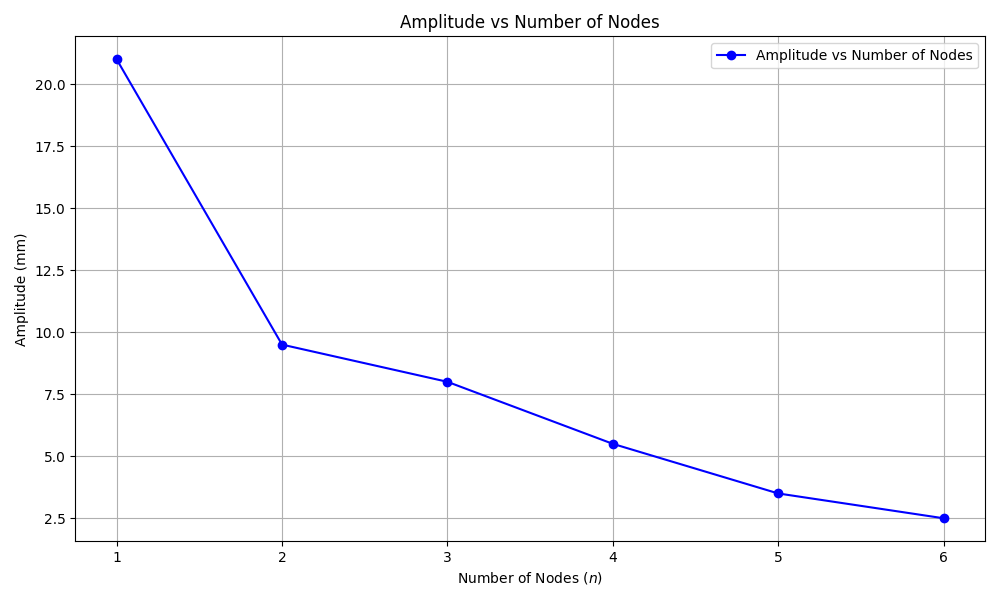
\includegraphics[width=4in]{images/amplitude1-6.png}
    \caption{Amplitude at $n=\{1\dots6\}$}
    \label{fig:amplitude}
\end{figure}

The velocity is constant, as we expect because it's not dependent on $f$ or $n$. See Figure \ref{fig:velocity}.

\begin{figure}[h]
    \centering
    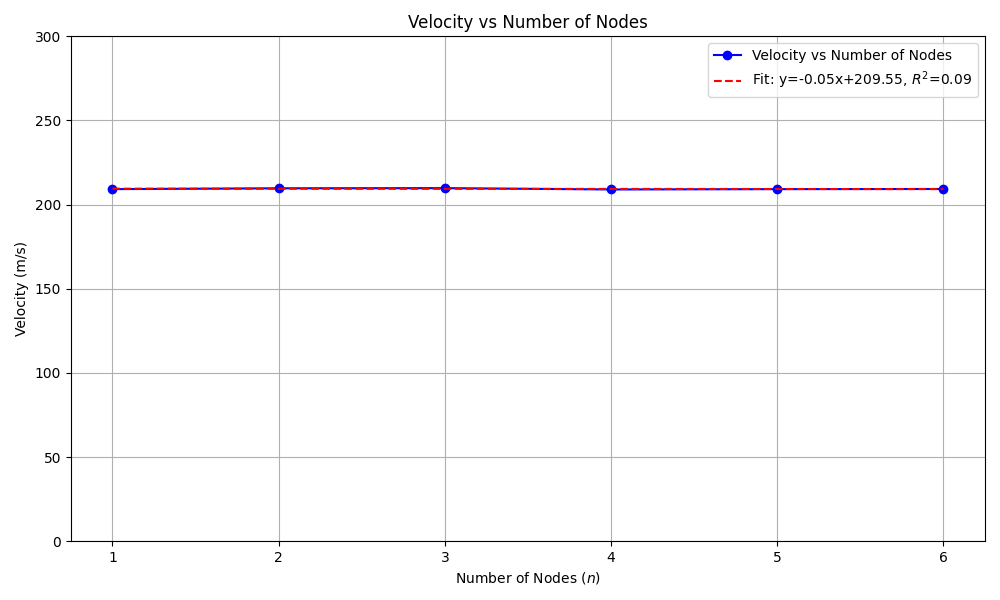
\includegraphics[width=4in]{images/velocity_vs_nodes.png}
    \caption{Velocity at $n=\{1\dots6\}$}
    \label{fig:velocity}
\end{figure}

\begin{table}[ht]
\centering
\begin{tabular}{lll}
                             & Frequency                            & Amplitude                        \\ \cline{2-3} 
\multicolumn{1}{l|}{0.343 N} & \multicolumn{1}{l|}{26.48 ± 0.01 Hz} & \multicolumn{1}{l|}{9.5 ± 1 mm}  \\ \cline{2-3} 
\multicolumn{1}{l|}{0.981 N} & \multicolumn{1}{l|}{45.48 ± 0.01 Hz} & \multicolumn{1}{l|}{11.5 ± 1 mm} \\ \cline{2-3} 
\multicolumn{1}{l|}{1.47 N}  & \multicolumn{1}{l|}{55.58 ± 0.01 Hz} & \multicolumn{1}{l|}{11 ± 1 mm}   \\ \cline{2-3} 
\multicolumn{1}{l|}{1.96 N}  & \multicolumn{1}{l|}{65.60 ± 0.01 Hz} & \multicolumn{1}{l|}{8 ± 1 mm}    \\ \cline{2-3} 
\multicolumn{1}{l|}{2.45 N}  & \multicolumn{1}{l|}{73.64 ± 0.01 Hz} & \multicolumn{1}{l|}{6.3 ± 1 mm}  \\ \cline{2-3} 
\multicolumn{1}{l|}{2.94 N}  & \multicolumn{1}{l|}{80.93 ± 0.01 Hz} & \multicolumn{1}{l|}{5.8 ± 1 mm}  \\ \cline{2-3} 
\multicolumn{1}{l|}{3.29 N}  & \multicolumn{1}{l|}{84.93 ± 0.01 Hz} & \multicolumn{1}{l|}{5 ± 1 mm}    \\ \cline{2-3} 
\end{tabular}
\label{tab:2n}
\caption{$n=2$ resonances at different tensions}
\end{table}

\begin{figure}[h]
    \centering
    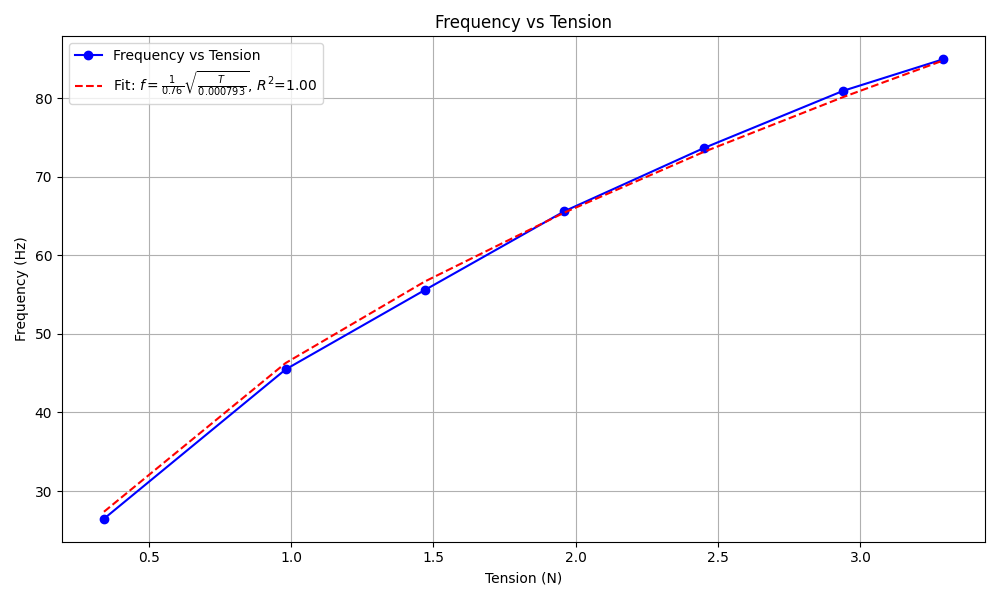
\includegraphics[width=4in]{images/tension_vs_frequency.png}
    \caption{Frequency at different tensions}
    \label{fig:tension}
\end{figure}

To find a relationship between tension and frequency, we need to understanding the relationship between tension and velocity, with the all important equation

\begin{equation}
\label{eqn:velocity}
    v= \sqrt{\frac{F}{\mu}}=\lambda f 
\end{equation}

We can get rid of v here, and rearrange to express frequency in terms of tension ($F$), wavelength ($\lambda$), and mass per unit length ($\mu$)!

\begin{equation*}
    f= \frac{1}{\lambda}\sqrt{\frac{F}{\mu}}
\end{equation*}

Doing a curve fit of such a function on our $n=2$ data, where we know $\lambda = 0.76 $ m, gives us an experimental $\mu = 0.000793 \frac{\text{kg}}{\text{m}}$. Unfortunately, we did not think to weigh our string, so we cannot verify this estimate. However, using it as a value gives a fit where $R^2 = 1.00$, which is excellent!


\section{Conclusions}

We found that there is a linear relationship between $n$ and frequency, which aligns with the theory. We have our basic wave equation

\begin{equation}
\label{eqn:wave}
    y(x,t)=A\cos\left(\omega\left(\frac{x}{v}-t\right)+\phi\right)
\end{equation}

And using some clever trigonometry tricks, we can rearrange this basic wave equation to solve for two waves. Since the length of the string is fixed, we can say it's a constant and $x=L$ To find a standing wave, let's set the equation for two waves we can set it equal to zero (which will give us waves with nodes):

\begin{equation}
\label{eqn:standing}
    y(L,t)=2A\sin\left(\frac{2\pi L}{\lambda}\right)\cos(\omega t)=0
\end{equation}

to solve this for a standing wave, it must be true that $\lambda=\frac{2L}{n}$ where $n \in \mathds{Z}$, which we observed. 

We also saw that the velocity was almost constant throughout our experiment, which makes sense, because it is not a function of $n$, but of force ($F$) and mass per unit length ($\mu$). See Equation \ref{eqn:velocity} and Figure \ref{fig:velocity}.

We also see that the relationship between tension and wavelength is as we expected (see Equation \ref{eqn:velocity} and Figure \ref{fig:tension}).

Waves work!


% \bibliographystyle{unsrtnat}
% \bibliography{references}

\end{document}
